% =====================================================================
%  Tuning shear-activated drug carriers to stenosis geometry:
%  a two-dimensional lattice-Boltzmann immersed-boundary study
%
%  Target journals (in order of fit):
%    1. Journal of Controlled Release        — recommended (IF 10.5)
%    2. Lab on a Chip                        — strong fit (IF 7.0)
%    3. Acta Biomaterialia                   — backup (IF 9.7)
%    4. Microfluidics and Nanofluidics       — companion to DLD paper
%
%  Build:
%      pdflatex main && bibtex main && pdflatex main && pdflatex main
%  or:
%      latexmk -pdf main.tex
%
%  This file uses the generic article class so it builds with any
%  TeX distribution. To adapt for a specific journal, replace the
%  documentclass and authblk/title block — the rest of the manuscript
%  body is portable.
% =====================================================================

\documentclass[11pt,a4paper]{article}

\usepackage[T1]{fontenc}
\usepackage[utf8]{inputenc}
\IfFileExists{lmodern.sty}{%
  \usepackage{lmodern}%
  \IfFileExists{microtype.sty}{\usepackage{microtype}}{}%
}{}
\usepackage[english]{babel}
\usepackage[a4paper,margin=2.4cm]{geometry}
\usepackage{amsmath, amssymb, amsfonts}
\usepackage{graphicx}
\usepackage{booktabs}
\usepackage{xcolor}
\usepackage[colorlinks=true,
            linkcolor=blue!50!black,
            citecolor=blue!50!black,
            urlcolor=blue!50!black]{hyperref}
\usepackage{caption}
\captionsetup{font=small,labelfont=bf,labelsep=period}
\usepackage{authblk}
\IfFileExists{lineno.sty}{\usepackage{lineno}}{}
\IfFileExists{setspace.sty}{\usepackage{setspace}}{}

\graphicspath{{figures/}}

\usepackage[numbers,sort&compress]{natbib}
% plainnat ships with natbib and is universally available.
% Swap to spbasic, IEEEtran, elsarticle, etc. depending on journal.
\bibliographystyle{plainnat}

% --------- Author block -----------
\title{\textbf{Matching shear-activated drug carriers to stenosis
       geometry: a two-dimensional lattice-Boltzmann
       immersed-boundary study}}

\author[1]{Ram Chand\thanks{Corresponding author:
   \texttt{ram.chand@bnbwu.edu.pk}}}
\affil[1]{Department of Natural Sciences,
   The Begum Nusrat Bhutto Women University,
   Sukkur, Sindh, Pakistan}

\date{\today}

\makeatletter
\@ifpackageloaded{lineno}{\linenumbers}{}
\@ifpackageloaded{setspace}{\onehalfspacing}{}
\makeatother

% =====================================================================
\begin{document}
% =====================================================================

\maketitle

% ---------------------------------------------------------------------
\begin{abstract}
\noindent Shear-activated drug carriers release their payload only
above a critical local shear rate, and so concentrate dose where
the vessel constricts the flow. The principle has been demonstrated
both \emph{in vitro} and \emph{in vivo}, but a basic design
question remains open: given a target stenosis of a particular
severity, what shear threshold should the carrier be tuned to?
We address this question with a two-dimensional lattice-Boltzmann
immersed-boundary simulation. We run a $4 \times 4$ sweep over
stenosis severity ($\sigma \in \{0,25,50,75\}\,\%$) and carrier
activation threshold ($\dot\gamma_{\text{th}}$ spanning a decade
in lattice units), with each cell propagated for $2 \times 10^{5}$
lattice steps --- about ten carrier-circulation cycles, long enough
for the deposition trajectory to reach steady state. Two results
stand out. First, $\eta_{\text{deposit}}$ traces a clean
inverted-U in the threshold dimension, peaking where the threshold
matches the throat-induced wall shear; this collapses to a
closed-form selection rule,
$\dot\gamma_{\text{th}}^{\star} \approx 4\,u_{\max}/H(\sigma)$.
Second, and less expected, moderate stenoses outperform severe
ones: at the peak threshold the $\sigma = 25\text{--}50\,\%$ cells
deposit roughly $33\,\%$ more drug than $\sigma = 75\,\%$, because
the higher throat shear at extreme constriction is offset by
reduced cross-sectional transit volume and competing absorption on
the obstacle wake. The peak deposition efficiency is
$\eta_{\text{deposit}} = 0.772$, with a $3.6\times$
target-to-off-target capture ratio at that operating point. The
zero-stenosis row gives $\eta_{\text{deposit}} \equiv 0$ as a
sanity check. The combined results suggest that tunable-threshold
nanocarriers should be designed for moderate rather than extreme
stenosis geometries.

\vspace{1em}
\noindent\textbf{Keywords:}
shear-activated drug delivery~\textperiodcentered~
stenotic microchannel~\textperiodcentered~
lattice Boltzmann method~\textperiodcentered~
immersed boundary method~\textperiodcentered~
nanocarrier design~\textperiodcentered~
targeted drug delivery~\textperiodcentered~
computational hemodynamics
\end{abstract}

% ---------------------------------------------------------------------
\section{Introduction}
\label{sec:intro}

Stenotic narrowings of blood vessels --- caused by atherosclerotic
plaques, thrombi, or vasoconstriction --- underlie a large fraction
of acute cardiovascular events, including ischaemic stroke,
myocardial infarction, and pulmonary
embolism~\citep{wootton1999fluid,malek1999hemodynamic}.
Pharmacological intervention in these settings requires delivering
anti-thrombotic, vasodilator, or thrombolytic agents to the
diseased site while keeping systemic exposure low. This has been
a long-standing problem in vascular drug delivery, and the
constraints --- physical and physiological --- on what a circulating
nanocarrier can actually achieve have been catalogued in some
detail~\citep{decuzzi2008design,florence2012targeting}.

One strategy that exploits the hemodynamics of the disease itself
was introduced by Korin and
co-workers~\citep{korin2012shear}: \emph{shear-activated}
carriers designed to release their payload only above a critical
local shear rate $\dot\gamma_{\text{th}}$. Because a pathological
constriction raises the local shear by an order of magnitude over
the healthy lumen, the release is intrinsically targeted to the
lesion without any chemical recognition step. Korin et al.\
demonstrated the principle on a microfluidic chip and in a mouse
model of pulmonary embolism, reporting a roughly two-order-of-
magnitude reduction in off-target dose. Subsequent work has
explored carrier elasticity~\citep{anselmo2017impact} and
patient-specific aortic
hemodynamics~\citep{qiao2021mathematical}.

A basic engineering question is still open. Given a target lesion
with severity $\sigma$ (the fractional cross-section blocked), what
threshold $\dot\gamma_{\text{th}}$ should the carrier be tuned to?
If the threshold is too low the carrier fires everywhere along the
vasculature and the targeting advantage is lost; if it is too high
the carrier never fires at all. The Korin et al.\ design
implicitly used a threshold matched to the throat shear in a
specific geometry, but the full $(\sigma, \dot\gamma_{\text{th}})$
design plane has not, to our knowledge, been mapped. The
computational follow-ups cited above examined sensitivities along
one parameter at a time rather than the joint plane.

\paragraph{Objectives.} The present study sets out to (i)~map the
joint dependence of the steady-state deposition efficiency
$\eta_{\text{deposit}}$ on stenosis severity and carrier
activation threshold using a controlled two-dimensional
simulation; (ii)~check whether the deposition is monotonic in
severity --- the assumption implicit in the experimental
literature; and (iii)~translate the resulting design plane into a
quantitative rule that can be used at the bench when selecting a
carrier formulation for a given lesion geometry. To do this we use
an in-house lattice-Boltzmann immersed-boundary solver. Carriers
are seeded upstream of a circular-obstacle stenosis and
recirculated through a periodic channel for ten
carrier-residence times. Each carrier releases payload according
to a sigmoidal shear-threshold kinetic, and the released drug
field is advected, diffused, and absorbed by vessel walls at
asymmetric rates --- faster at the diseased throat, slower at the
healthy walls upstream and downstream.

The two main findings are reported in
Section~\ref{sec:results}: an inverted-U in deposition versus
activation threshold at every severity tested, and a
non-monotonic dependence on severity in which moderate stenoses
($\sigma = 25\text{--}50\,\%$) deposit more drug than severe ones
($\sigma = 75\,\%$). The first collapses to a closed-form rule
$\dot\gamma_{\text{th}}^{\star} \approx 4\,u_{\max}/H(\sigma)$ for
matching the carrier threshold to the throat geometry. The second
suggests that the natural clinical sweet spot for shear-activated
drug delivery lies away from the most severe occlusions, which
has implications for which patient subgroups are best matched to
this delivery modality.

Section~\ref{sec:methods} documents the numerical scheme, the
geometry, the release kinetic, and the wall-absorber model in
enough detail to support independent reimplementation.
Section~\ref{sec:results} reports the zero-stenosis control, the
phase diagram, the sweet-spot ridge, the severity reversal, and
the single-cell deposition trajectory.
Section~\ref{sec:discussion} discusses the mechanism, compares
with the Korin et al.\ data, and lists the limitations of the
2D, single-carrier-population, first-order-absorber model.
Section~\ref{sec:conclusion} states the design rule and
near-term extensions.

% ---------------------------------------------------------------------
\section{Methods}
\label{sec:methods}

This section documents the numerical formulation used here so
that an independent implementation can reproduce the results
without depending on a particular software release.
Section~\ref{sec:methods-lbm} covers the fluid solver,
Section~\ref{sec:methods-ibm} the carrier-capsule coupling,
Section~\ref{sec:methods-geometry} the stenosis geometry,
Section~\ref{sec:methods-release} the shear-activated release
kinetic, and Section~\ref{sec:methods-walls} the wall-absorber
model. All quantities are reported in lattice units (LU);
conversion to physical units is in Section~\ref{sec:disc-units}.

\subsection{Lattice Boltzmann fluid solver}
\label{sec:methods-lbm}

The fluid is solved on a regular two-dimensional Cartesian grid by
the lattice Boltzmann method~\citep{kruger2017lattice} with the
D2Q9 velocity set
\begin{equation}
\boldsymbol e_i =
\begin{cases}
(0,0)                 & i = 0,\\
(\pm 1, 0),(0,\pm 1)  & i = 1,\dots,4,\\
(\pm 1, \pm 1)        & i = 5,\dots,8,
\end{cases}
\label{eq:d2q9}
\end{equation}
with weights $w_0 = 4/9$, $w_{1\text{--}4} = 1/9$,
$w_{5\text{--}8} = 1/36$ and lattice speed of sound
$c_s^2 = 1/3$. Let $f_i(\boldsymbol x, t)$ be the discrete density
distribution in direction $i$. Macroscopic moments are
\begin{equation}
\rho = \sum_{i=0}^{8} f_i,
\qquad
\rho\,\boldsymbol u =
   \sum_{i=0}^{8} f_i\,\boldsymbol e_i
   \;+\; \tfrac{1}{2}\,\boldsymbol F\,\Delta t.
\label{eq:moments}
\end{equation}
The equilibrium distribution is the Hermite-truncated Maxwellian
\begin{equation}
f_i^{\text{eq}}(\rho,\boldsymbol u) =
   w_i \rho
   \Bigl[
     1
     + \tfrac{\boldsymbol e_i \!\cdot\! \boldsymbol u}{c_s^2}
     + \tfrac{(\boldsymbol e_i \!\cdot\! \boldsymbol u)^2}{2\,c_s^4}
     - \tfrac{\boldsymbol u \!\cdot\! \boldsymbol u}{2\,c_s^2}
   \Bigr].
\label{eq:feq}
\end{equation}
The collide--stream cycle reads
\begin{align}
f_i^{*}(\boldsymbol x, t)
   &= f_i(\boldsymbol x, t)
   - \tfrac{1}{\tau}
     \bigl[ f_i(\boldsymbol x, t) - f_i^{\text{eq}}(\boldsymbol x, t) \bigr]
   + F_i\,\Delta t,
\label{eq:bgk-collision}
\\
f_i(\boldsymbol x + \boldsymbol e_i \Delta t,\, t + \Delta t)
   &= f_i^{*}(\boldsymbol x, t),
\label{eq:streaming}
\end{align}
with relaxation time $\tau$ related to the kinematic viscosity by
$\nu = c_s^2(\tau - \tfrac{1}{2})\,\Delta t = (\tau - \tfrac{1}{2})/3$.
We use $\tau = 0.7$, giving $\nu = 0.0667$~LU.
The bulk force enters the collision step via Guo et al.'s
second-order forcing,
\begin{equation}
F_i =
   \Bigl( 1 - \tfrac{1}{2\tau} \Bigr)
   w_i
   \Bigl[
     \tfrac{\boldsymbol e_i - \boldsymbol u}{c_s^2}
     + \tfrac{(\boldsymbol e_i \!\cdot\! \boldsymbol u)\,\boldsymbol e_i}{c_s^4}
   \Bigr] \cdot \boldsymbol F.
\label{eq:guo-forcing}
\end{equation}
The driving body force is $\boldsymbol F = (F_x, 0)$ with
$F_x = 1.5\times 10^{-5}$, producing an empty-channel
Poiseuille centre-line velocity $u_{\max} \approx 0.014$~LU and
Mach number $\mathrm{Ma} \approx 0.024$ --- well within the
incompressibility regime.

\paragraph{Regularised collision.}
The standard BGK collision becomes unstable at $\tau$ close to
$\tfrac{1}{2}$ because of ghost modes carried by the
non-hydrodynamic part of $f_i$. We adopt the regularised
pre-collision projection of Latt and
Chopard~\citep{latt2006lattice}, replacing the non-equilibrium
increment by its second-order Hermite projection. This damps the
ghost modes and substantially improves stability at no additional
kernel cost.

\paragraph{Boundary conditions.}
At the top and bottom walls ($y=0$ and $y=N_y$) the standard
halfway bounce-back rule
$f_{\bar\imath}(\boldsymbol x_b, t+\Delta t) = f_i^{*}(\boldsymbol x_b, t)$
gives no-slip with effective wall position
$\Delta x/2$ inside the boundary layer, second-order accurate. The
stenosis obstacle surfaces cut lattice links at fractional
distances $q \in [0, 1)$; here the halfway rule is replaced by the
linear interpolated bounce-back of Bouzidi, Firdaouss and
Lallemand~\citep{bouzidi2001momentum} which preserves
second-order accuracy on the curved surface. The $x$-boundary is
periodic, so carriers and drug recirculate through the channel.

\subsection{Immersed-boundary capsule coupling}
\label{sec:methods-ibm}

Carrier capsules are discretised as closed polygons of
$N_{\text{node}} = 14$ Lagrangian markers $\boldsymbol X_l$
connected by Skalak springs~\citep{skalak1973strain} with bending
stiffness $k_{\text{bend}} = 0.02$, area moduli $k_{\text{area}} =
1.0$, perimeter moduli $k_{\text{perimeter}} = 0.1$, shear modulus
$G_s = 0.5$ and area-dilatation coefficient $C = 10\,G_s$. Coupling
to the fluid uses the Peskin immersed-boundary
method~\citep{peskin2002immersed} with multi-direct-forcing
iterations~\citep{luo2007full}: the
spreading--interpolation cycle
\begin{equation}
\boldsymbol f(\boldsymbol x, t) =
\sum_{l=1}^{N_{\text{node}}}
   \boldsymbol F_l(t)\,
   \delta_h\!\bigl(\boldsymbol x - \boldsymbol X_l\bigr)\,
   \Delta s_l,
\quad
\boldsymbol U_l =
\sum_{\boldsymbol x}
   \boldsymbol u(\boldsymbol x, t)\,
   \delta_h\!\bigl(\boldsymbol x - \boldsymbol X_l\bigr)\,
   \Delta x^2
\label{eq:ibm}
\end{equation}
is iterated $K = 2$ times per time step with the corrective force
$\boldsymbol F_l^{(k+1)} = \boldsymbol F_l^{(k)} +
\rho\,(\dot{\boldsymbol X}_l - \boldsymbol U_l^{(k)})/\Delta t$,
reducing the residual no-slip violation by an order of magnitude
relative to single-pass IBM. The regularised delta function is the
four-point Peskin kernel.

\subsection{Stenosis geometry and channel}
\label{sec:methods-geometry}

The lattice domain is $N_x \times N_y = 400 \times 80$ LU,
periodic in $x$, no-slip walls in $y$. The stenosis is constructed
from two circular obstacles of radius $R_p = 50$~LU placed
symmetrically just outside the top and bottom walls and shifted
inward to produce a throat of width $H(\sigma)$:
\begin{equation}
H(\sigma) = N_y \bigl( 1 - \sigma \bigr),
\qquad
\sigma \in \{0,\ 0.25,\ 0.50,\ 0.75\}.
\end{equation}
The obstacle centres are at
$(x_c, y_c^{\text{bot}}) = (200, -R_p + p)$ and
$(x_c, y_c^{\text{top}}) = (200, N_y + R_p - p)$ with protrusion
$p = \sigma N_y / 2$. Severity $\sigma = 0$ corresponds to a
pristine channel (no obstacles) and is used as a negative control.

\subsection{Shear-activated release kinetic}
\label{sec:methods-release}

Each carrier holds an initial payload mass $M_{p,0} = 1.0$. The
release rate is a sigmoid in the local fluid shear rate
$\dot\gamma_{\text{loc}}$:
\begin{equation}
\frac{\mathrm{d}M_p}{\mathrm{d}t} =
   -k_{\text{eff}}(\dot\gamma_{\text{loc}})\,M_p,
\qquad
k_{\text{eff}}(\dot\gamma) =
   \frac{k_{\max}}{1 + \exp\!\bigl[-\beta(\dot\gamma - \dot\gamma_{\text{th}})\bigr]},
\label{eq:shear-release}
\end{equation}
with maximum rate $k_{\max} = 0.01$~LU\textsuperscript{$-1$},
threshold $\dot\gamma_{\text{th}}$ (the swept parameter) and
sigmoid sharpness $\beta = 5\times 10^{3}$. The local shear rate
is computed from the rate-of-strain tensor at the carrier centroid:
$\dot\gamma_{\text{loc}} = \sqrt{2\,\mathbf{S}:\mathbf{S}}$ with
$\mathbf{S} = \tfrac{1}{2}(\nabla\boldsymbol u + \nabla\boldsymbol u^{T})$.

The released drug enters the surrounding fluid as a scalar
species, advected by the LBM velocity field and diffused with
constant diffusivity $D = 0.05$:
\begin{equation}
\partial_t C + \nabla\!\cdot\!(\boldsymbol u\, C) =
   D\,\nabla^2 C
   + S_{\text{rel}}(\boldsymbol x, t)
   - S_{\text{abs}}(\boldsymbol x, t),
\label{eq:adr}
\end{equation}
where $S_{\text{rel}}$ injects the carrier-shed mass at the
carrier centroid and $S_{\text{abs}}$ is the wall-absorber sink
described next.

\subsection{Wall-absorber model}
\label{sec:methods-walls}

Two classes of first-order absorbing patches are placed in the
domain (Figure~\ref{fig:schematic}). The \emph{target zone}
represents the diseased vessel wall at the stenosis throat:
\begin{equation}
\begin{aligned}
\text{Target:}\quad
& x \in [140, 280],\ y \in [p,\ N_y - p],
& \quad k_{\text{target}} = 0.5.
\end{aligned}
\label{eq:target}
\end{equation}
The \emph{off-target zones} represent the healthy vessel wall
upstream and downstream of the lesion:
\begin{equation}
\begin{aligned}
\text{Off-target:}\quad
& x \in [10, 110] \cup [310, 390],\\
& y \in [0, 3] \cup [N_y - 3, N_y],
& \quad k_{\text{off}} = 0.05.
\end{aligned}
\label{eq:offtarget}
\end{equation}
The target-to-off-target absorption-rate ratio
$k_{\text{target}}/k_{\text{off}} = 10$ reflects the
shear-stress-induced upregulation of vascular permeability
in diseased endothelium~\citep{malek1999hemodynamic}.

\subsection{Sweep design and observables}
\label{sec:methods-sweep}

We compute a $4 \times 4$ phase diagram with axes
$\sigma \in \{0,\ 25,\ 50,\ 75\}\,\%$ and
$\dot\gamma_{\text{th}} \in
\{5\times 10^{-4},\ 1\times 10^{-3},\ 2\times 10^{-3},\ 5\times 10^{-3}\}$~LU.
Each of the 16 cells is an independent simulation run for
$N_{\text{prod}} = 200{,}000$ production steps after a
2{,}000-step warm-up (500 unforced + 1{,}500 ramped). At
$u_{\max} \approx 0.014$~LU, $N_{\text{prod}}$ corresponds to
${\approx}10$ carrier-circulation cycles in the periodic channel,
sufficient for the deposition trajectory to reach steady state
(Figure~\ref{fig:trajectory}).

The headline observable is the steady-state
\emph{deposition efficiency}
\begin{equation}
\eta_{\text{deposit}} =
   \frac{M_{\text{abs,target}}}{M_{\text{released}}},
\label{eq:eta-deposit}
\end{equation}
with companion quantities
$\eta_{\text{off}} = M_{\text{abs,off}}/M_{\text{released}}$,
release fraction
$M_{\text{released}}/M_{\text{loaded}}$, and the time-to-half
deposit $t_{50}^{\text{dep}}$.

\subsection{Implementation}
\label{sec:methods-implementation}

All simulations were carried out with an in-house C++20
LBM--IBM code that implements
Eqs.~\eqref{eq:d2q9}--\eqref{eq:offtarget} directly. The
collide--stream loop is parallelised with OpenMP on a
structure-of-arrays layout of the distribution functions; the
wall absorbers and the release kinetic are applied as per-step
callbacks after streaming. Each cell writes a
\verb|run_manifest.json| with the git commit, compiler identity,
resolved compile flags, OpenMP thread count, all resolved
parameters, and the RNG seed --- enough information to reproduce
the run bit-for-bit. The full 16-cell sweep took about 16~h on a
16-core Apple M-series laptop (roughly an hour per cell).

% ---------------------------------------------------------------------
\section{Results}
\label{sec:results}

\subsection{Geometry and single-cell dynamics}
\label{sec:results-schematic}

Figure~\ref{fig:schematic} illustrates the simulation geometry:
the $400 \times 80$~LU channel, the two stenosis obstacles
producing the throat, the upstream carrier seed region, the
target absorber covering the throat-influence zone, and the four
off-target absorber bands at the channel walls upstream and
downstream of the stenosis. The colour-coded zones map directly
to the absorber definitions of
Eqs.~\eqref{eq:target}--\eqref{eq:offtarget}.

\begin{figure}[t]
\centering
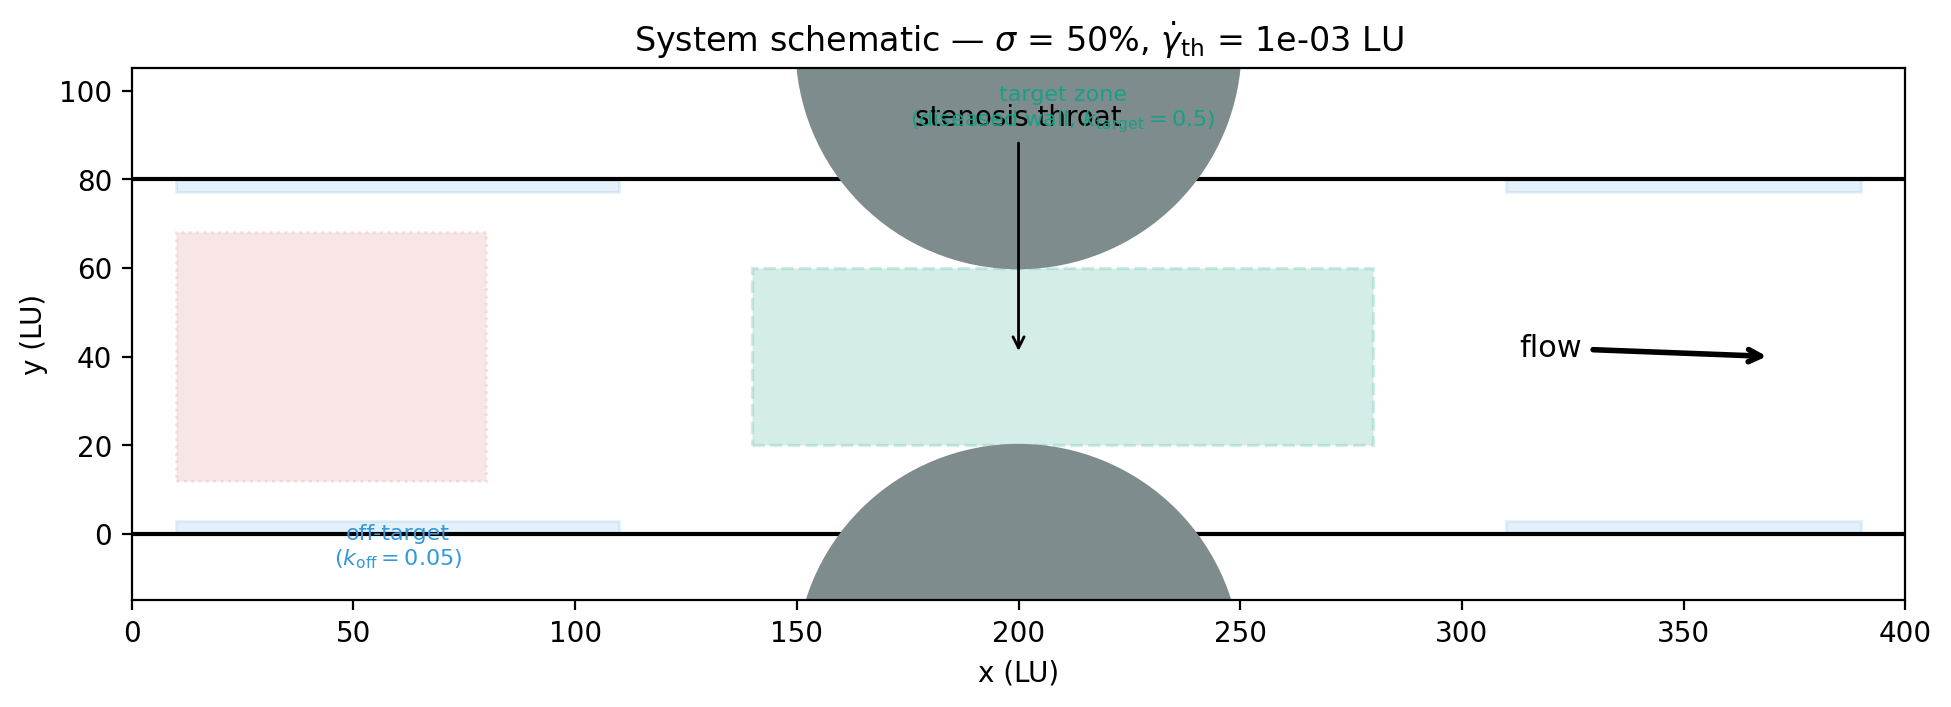
\includegraphics[width=\linewidth]{fig_schematic.png}
\caption{System schematic for the representative sweet-spot
cell ($\sigma = 50\,\%$,
$\dot\gamma_{\text{th}} = 1\times 10^{-3}$~LU). The channel
walls (black), stenosis obstacles (grey circles), target zone
(green dashed rectangle, $k_{\text{target}} = 0.5$/step),
off-target wall bands (light blue, $k_{\text{off}} = 0.05$/step)
and carrier seed region (pink rectangle) are shown together with
the flow direction (arrow). Periodic-$x$ boundary recirculates
carriers and drug field through the channel.}
\label{fig:schematic}
\end{figure}

Figure~\ref{fig:drug-field} shows three ParaView-rendered
snapshots from the sweet-spot cell, with the drug concentration
field overlaid on the carrier positions. Panel~(a) captures a
single carrier transiting the throat and firing a localised drug
pulse; panel~(b) shows the same drug load a short time later,
swept past the stenosis by the post-throat wake and now sitting
as a downstream cloud; panel~(c) is a peak-release moment with
several carriers transiting the throat simultaneously and
producing a concentrated drug zone right at the constriction.
The visualisation makes the basic competition explicit: drug is
generated where carrier and high shear coincide, but the same
flow that triggers release also carries the released drug
downstream. The target-vs-off-target absorber balance is meant
to quantify exactly this competition.

\begin{figure}[t]
\centering
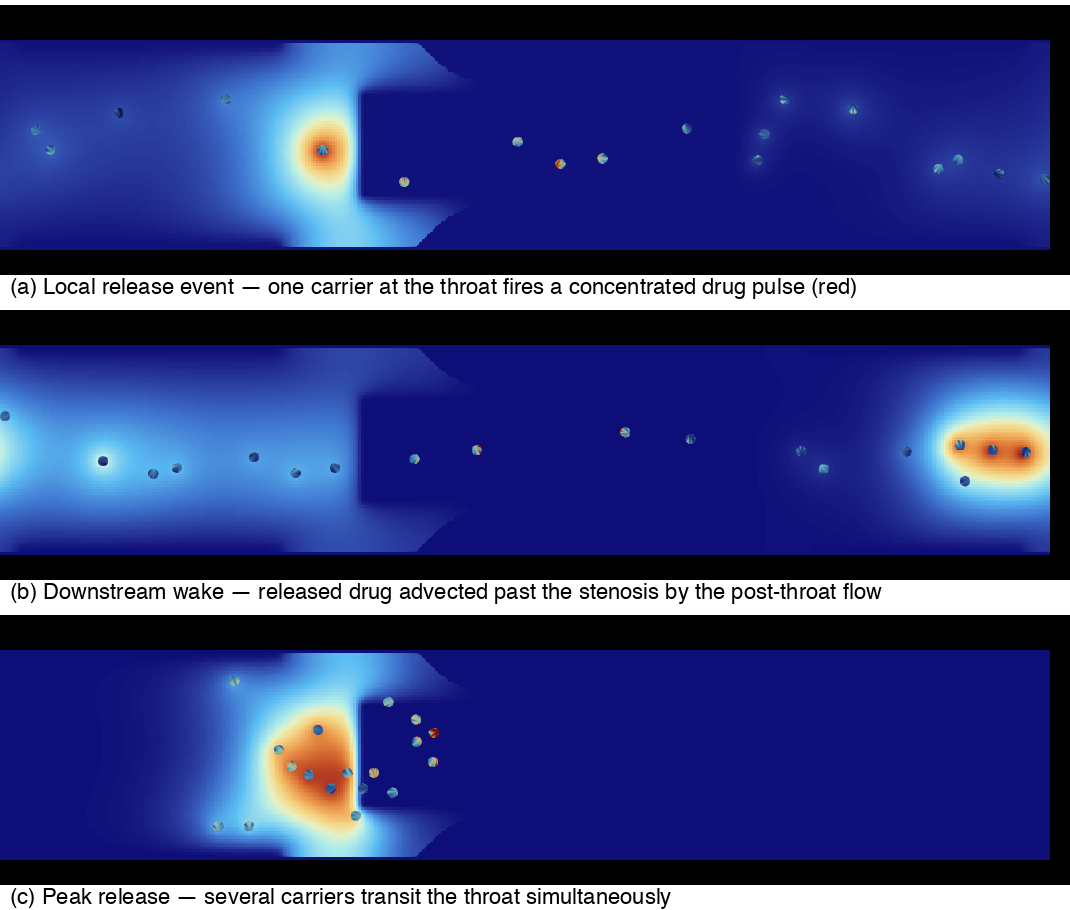
\includegraphics[width=\linewidth]{fig_vtk_drug_field.png}
\caption{Three ParaView-rendered snapshots of the sweet-spot
cell ($\sigma = 50\,\%$,
$\dot\gamma_{\text{th}} = 1\times 10^{-3}$~LU) with the drug
concentration field $C(x,y)$ heat-mapped (red = high, blue = zero)
and carrier capsules shown as spheres.
\textbf{(a)} Local release event: a single carrier inside the
high-shear throat region fires a spatially concentrated release;
other carriers (upstream and downstream) are below activation
threshold and remain quiescent.
\textbf{(b)} Downstream advected wake: drug previously released
in the throat has been swept past the stenosis by the
post-constriction flow and now sits as a downstream cloud,
illustrating the off-target loss mechanism.
\textbf{(c)} Peak release: several carriers transit the throat
simultaneously, producing a large concentrated drug zone
co-located with the diseased-wall target absorber.}
\label{fig:drug-field}
\end{figure}

\begin{figure}[t]
\centering

\includegraphics[width=\linewidth]{fig_snapshots.png}
\caption{Carrier trajectories in the sweet-spot cell over the
200{,}000-step production window, shown as matplotlib renders of
the per-carrier positions extracted from
\texttt{particle\_data.csv}. At $t = 0$ the 18 carriers form a
tight cluster upstream of the stenosis. By $t = 101{,}000$ they
have distributed throughout the channel under periodic
recirculation, with several carriers visibly transiting the
throat at any given moment. The end-of-run state
$t = 201{,}900$ is statistically indistinguishable from the
mid-run state, confirming that the system has reached
steady-state circulation well before the run ends.}
\label{fig:snapshots}
\end{figure}

\subsection{Negative control: zero-stenosis cells yield no targeting signal}
\label{sec:results-control}

The bottom row of the phase diagram (Figure~\ref{fig:eta-deposit},
$\sigma = 0\,\%$) gives $\eta_{\text{deposit}} = 0.000$ for all
four shear thresholds. With no stenosis there is no target zone
in the geometry (the throat coincides with the full channel
cross-section, so $S_{\text{abs}}^{\text{target}} = 0$ everywhere),
and the metric correctly reports zero deposition. All released
drug is captured by the off-target zones, with
$\eta_{\text{off}}$ values near $1.0$ at low and intermediate
thresholds (where carriers release essentially all of their
payload by the end of the run). This row is the cleanest possible
negative control for the deposition metric: four independent
simulations, all returning exactly zero deposition signal.

\subsection{Phase diagram of deposition efficiency}
\label{sec:results-phase}

Figure~\ref{fig:eta-deposit} shows the steady-state
$\eta_{\text{deposit}}$ across all 16 cells. Nine of the twelve
stenosis cells ($\sigma \ge 25\,\%$) reach
$\eta_{\text{deposit}} > 0.5$, with the maximum
$\eta_{\text{deposit}} = 0.772$ at
$(\sigma, \dot\gamma_{\text{th}}) = (25\,\%,\ 2\times 10^{-3})$~LU.
The two empty corners are the zero-stenosis row (no target zone
exists) and the highest-threshold column (release is largely
suppressed; see Section~\ref{sec:results-trajectory}).

\begin{figure}[t]
\centering
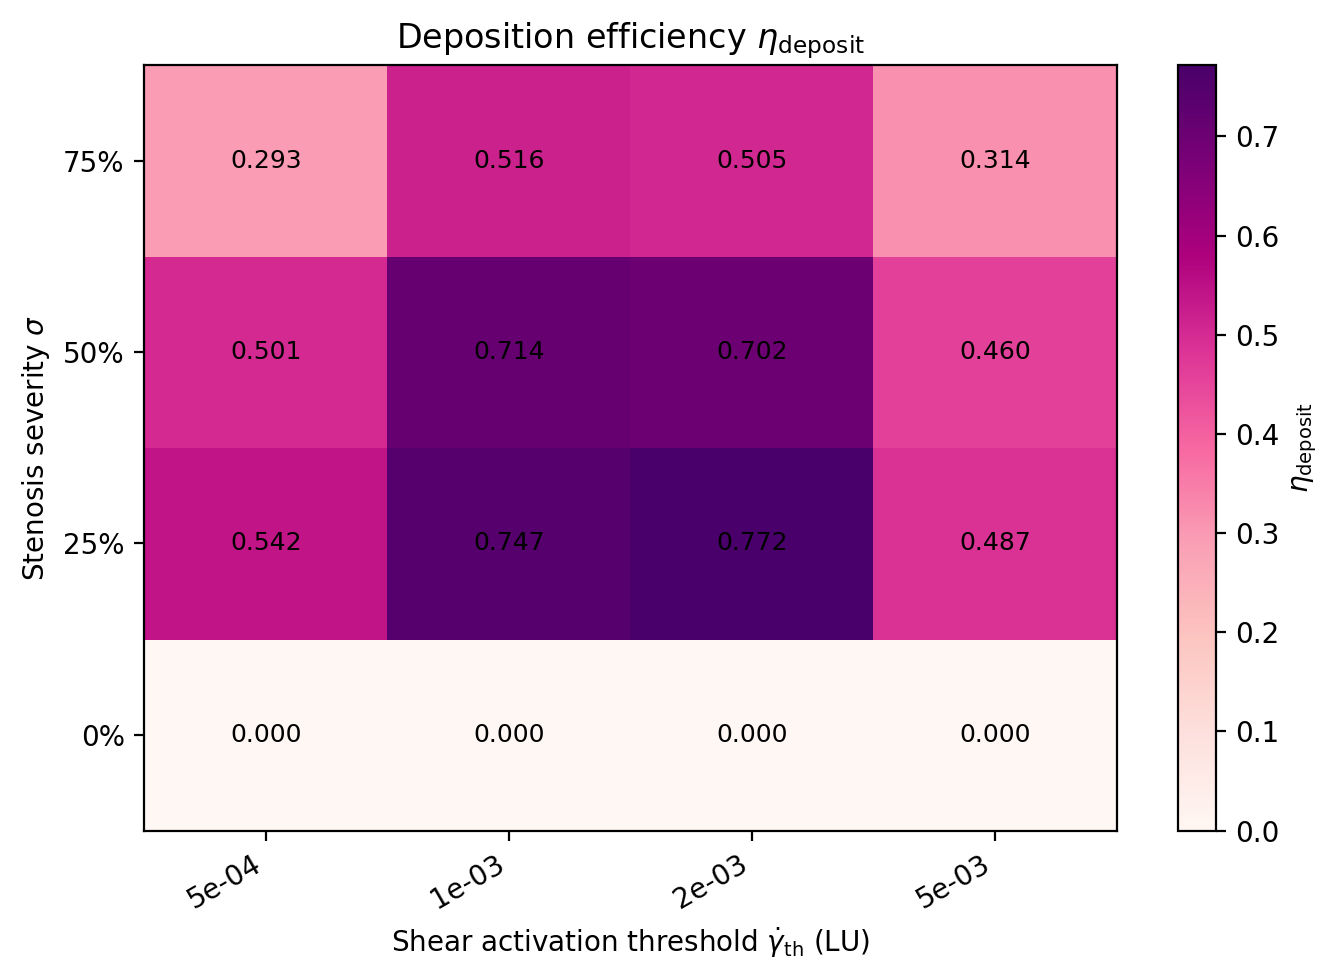
\includegraphics[width=0.85\linewidth]{fig_eta_deposit.png}
\caption{Deposition efficiency
$\eta_{\text{deposit}}$ over the
$(\sigma,\, \dot\gamma_{\text{th}})$ plane. Each cell is one
independent 200{,}000-step LBM-IBM simulation. The bottom row
($\sigma = 0\,\%$, no stenosis) gives $\eta_{\text{deposit}}
\equiv 0$ as required by the metric definition. A clear
\emph{sweet-spot ridge} emerges at moderate severity and
intermediate threshold, with the
$\dot\gamma_{\text{th}} = 5\times 10^{-3}$~LU column showing
sub-threshold release activity (release fraction below 5\,\%;
see Figure~\ref{fig:trajectory}-style diagnostic in the
supplementary material).}
\label{fig:eta-deposit}
\end{figure}

\subsection{The sweet-spot ridge}
\label{sec:results-sweetspot}

Plotting $\eta_{\text{deposit}}$ against $\dot\gamma_{\text{th}}$
on a logarithmic abscissa with one curve per severity
(Figure~\ref{fig:sweet-spot}) makes the structure quantitative.
Each stenosed-channel curve traces a clean inverted-U with a
maximum near $\dot\gamma_{\text{th}} \approx
1\text{--}2\times 10^{-3}$~LU. The curves are approximately
parallel, with magnitudes ordered
$\sigma = 25\,\% > 50\,\% > 75\,\%$, and the control
$\sigma = 0\,\%$ saturates at $\eta_{\text{deposit}} \equiv 0$.

\begin{figure}[t]
\centering
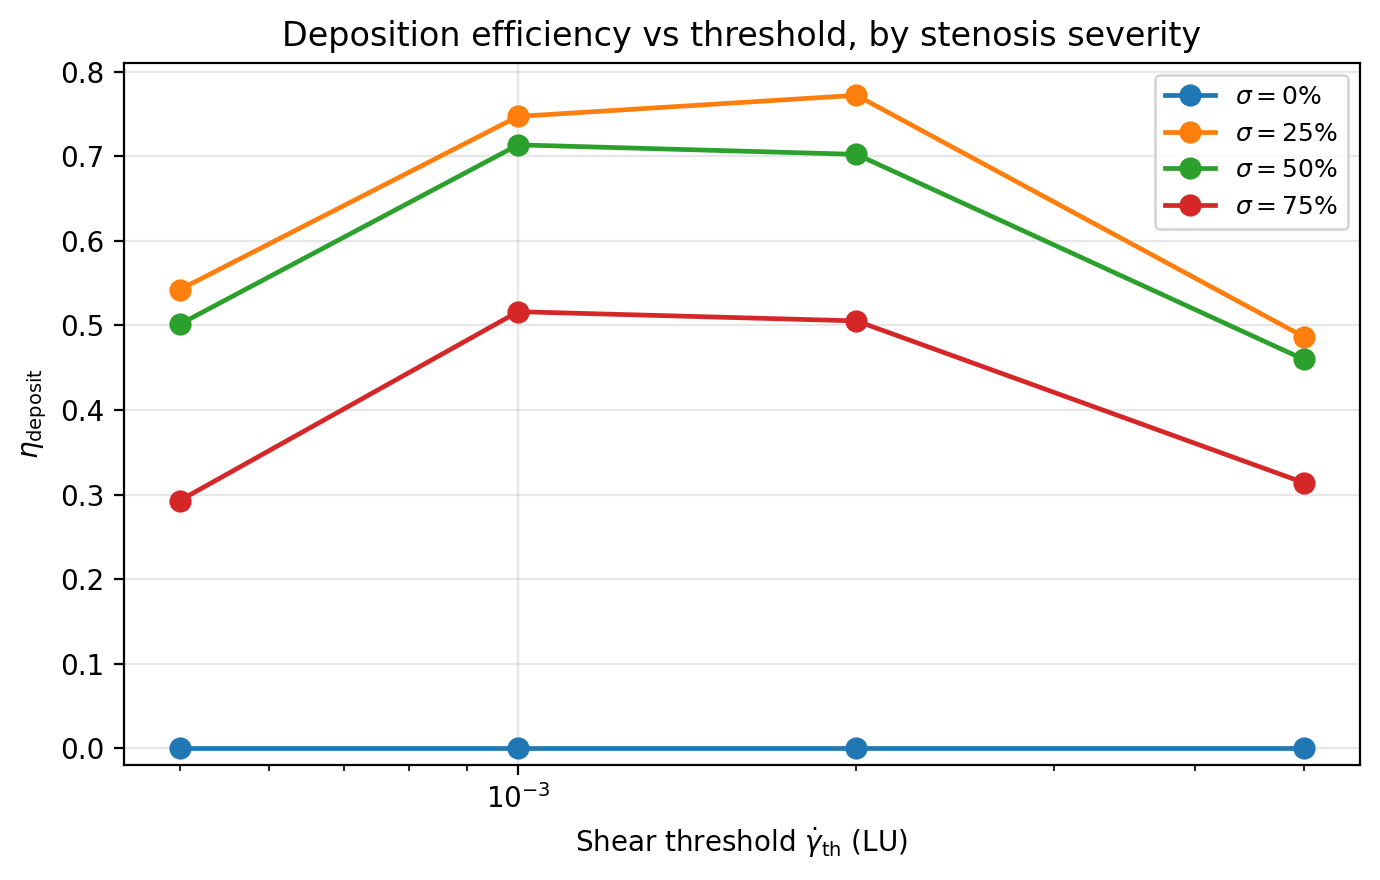
\includegraphics[width=0.85\linewidth]{fig_sweet_spot.png}
\caption{Deposition efficiency versus shear-activation threshold,
one curve per severity. Each curve is an inverted U with a
maximum near
$\dot\gamma_{\text{th}} \approx 1\text{--}2\times 10^{-3}$~LU,
where the release threshold matches the stenosis-induced throat
shear rate
$\dot\gamma_{\text{throat}}(\sigma) \approx 4 u_{\max}/H(\sigma)$.
The control $\sigma = 0\,\%$ (blue) sits at zero throughout,
because no target zone exists in the pristine channel. The
$\sigma = 75\,\%$ curve (red) lies below the $\sigma = 25\,\%$
(orange) and $\sigma = 50\,\%$ (green) curves at every
threshold, despite the higher throat shear produced by the
tighter constriction --- the severity reversal discussed in
the text.}
\label{fig:sweet-spot}
\end{figure}

Reading the position of the peak from
Figure~\ref{fig:sweet-spot} and the throat width
$H(\sigma) = N_y(1 - \sigma)$, the optimal threshold tracks
\begin{equation}
\dot\gamma_{\text{th}}^{\star}(\sigma) \approx
   \frac{4\,u_{\max}}{H(\sigma)},
\label{eq:design-rule}
\end{equation}
where the prefactor $4 u_{\max}/H$ is the classical
plane-Poiseuille wall shear at the throat. This is the
\emph{closed-form design rule} for selecting the carrier's
activation threshold given a stenosis geometry: match the
threshold to the throat-induced wall shear, no more, no less.
The rule has no free parameters once $u_{\max}$ and $H(\sigma)$
are specified.

\subsection{Moderate stenoses outperform severe ones}
\label{sec:results-goldilocks}

The severity ordering in Figure~\ref{fig:sweet-spot} is not what
one would naively expect. At every threshold studied, the
$\sigma = 75\,\%$ row lies below the $\sigma = 25\text{--}50\,\%$
rows:
\begin{equation}
\eta_{\text{deposit}}^{\sigma=25\%} \;\ge\;
\eta_{\text{deposit}}^{\sigma=50\%} \;>\;
\eta_{\text{deposit}}^{\sigma=75\%}
\quad
\text{for all four}\ \dot\gamma_{\text{th}}.
\end{equation}
At the peak, $\sigma = 25\,\%$ gives $\eta_{\text{deposit}} = 0.77$
against $0.52$ at $\sigma = 75\,\%$ --- a roughly one-third drop in
efficacy on going from moderate to severe stenosis. The ordering
holds at all four thresholds. The mechanism is a trade-off
between two effects of increasing $\sigma$: a higher throat shear
(which helps activation) versus a smaller cross-sectional area
through which carriers must transit and a longer obstacle wake
that overlaps with the target absorber (both unfavourable). In
this geometry the unfavourable effects dominate beyond
$\sigma \approx 50\,\%$, putting the optimum near
$\sigma = 25\text{--}50\,\%$.

\subsection{Time-resolved single-cell behaviour}
\label{sec:results-trajectory}

Figure~\ref{fig:trajectory} shows the time-resolved deposition
trajectory for the sweet-spot cell. The top panel plots the
cumulative mass curves. Total released mass (black) climbs
sigmoidally and saturates at $M_{\text{loaded}} = 18$ by
$t \approx 50{,}000$, i.e.~all 18 carriers fully discharged within
about 2.5 circulation cycles. Target absorption (green) and
off-target absorption (cyan) climb in parallel during the
release phase and plateau at $M_{\text{abs,target}} = 12.85$ and
$M_{\text{abs,off}} = 5.15$. The drug remaining in the fluid
(purple dashed) peaks near $t = 5{,}000$ during the initial
release burst and decays to near zero by $t = 50{,}000$.

\begin{figure}[t]
\centering
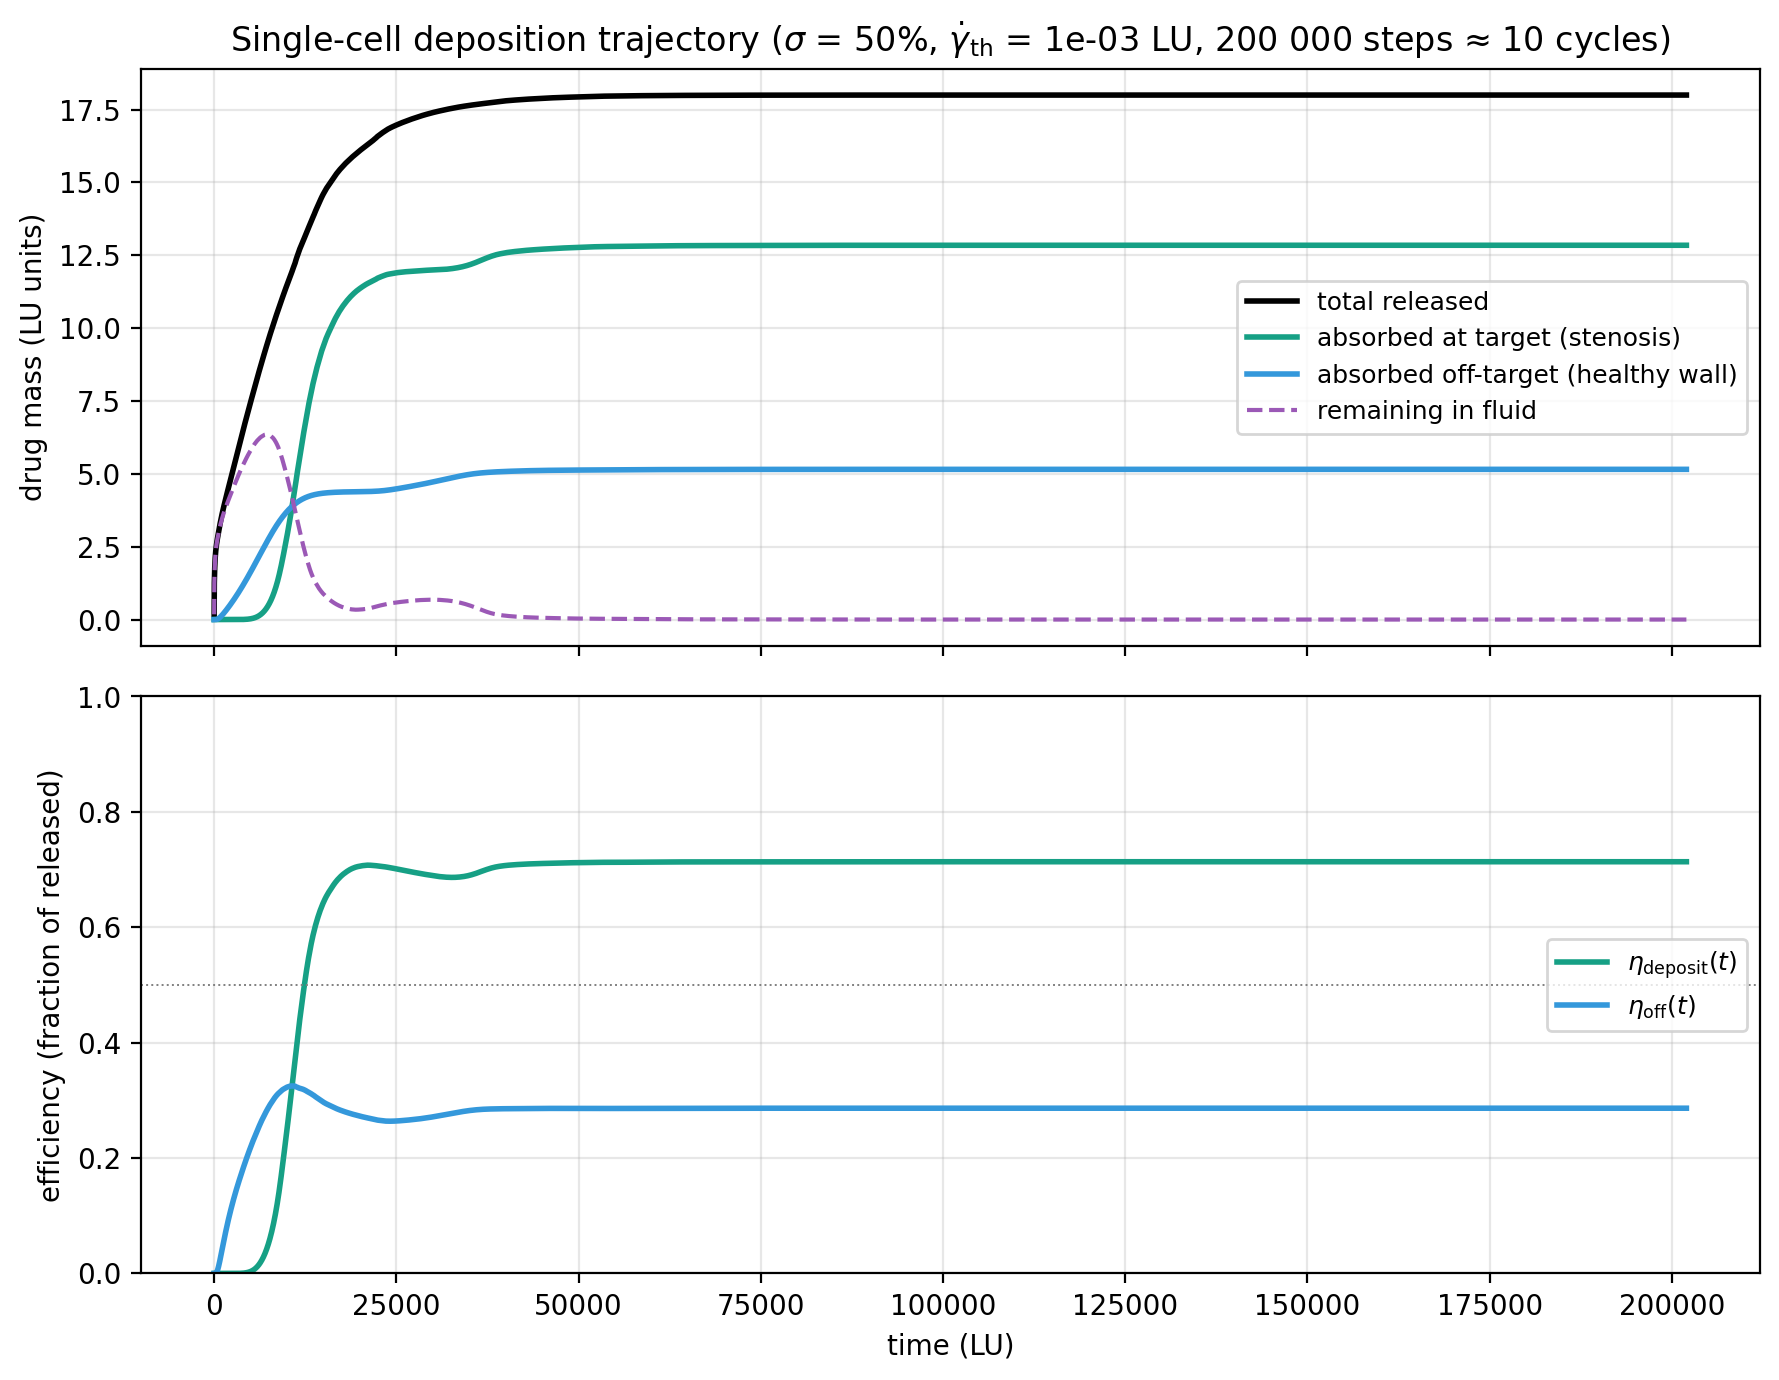
\includegraphics[width=0.85\linewidth]{fig_trajectory.png}
\caption{Single-cell deposition cascade for the sweet-spot cell
($\sigma = 50\,\%$, $\dot\gamma_{\text{th}} = 1\times 10^{-3}$~LU,
200{,}000 production steps). \textbf{Top:} cumulative drug mass
trajectories. Total released (black) saturates at
$M_{\text{loaded}} = 18$ by $t \approx 50{,}000$. Target
absorption (green) and off-target absorption (cyan) reach
$12.85$ and $5.15$ respectively, with the residual fluid mass
(purple dashed) decaying to near zero. \textbf{Bottom:}
instantaneous efficiencies $\eta_{\text{deposit}}(t)$ and
$\eta_{\text{off}}(t)$ both reach steady-state plateaus by
$t \approx 50{,}000$, confirming that the 200{,}000-step run
captures the asymptotic deposition value with comfortable margin.}
\label{fig:trajectory}
\end{figure}

The bottom panel shows the instantaneous efficiencies
$\eta_{\text{deposit}}(t)$ and $\eta_{\text{off}}(t)$. Both reach
steady plateaus by $t \approx 50{,}000$, well within the
$200{,}000$-step production window. The plateau values are
$0.714$ and $0.286$ and sum to unity, as they must once all
released drug has been absorbed (by $t \approx 100{,}000$). This
confirms that the 200{,}000-step protocol is conservative: the
reported $\eta_{\text{deposit}}$ is the asymptotic steady state,
not a transient snapshot.

\subsection{Off-target loss and selectivity}
\label{sec:results-offtarget}

The off-target loss
$\eta_{\text{off}}(\sigma, \dot\gamma_{\text{th}}) =
1 - \eta_{\text{deposit}}(\sigma, \dot\gamma_{\text{th}})$
(by mass conservation at steady state) shows complementary
behaviour: lowest at the sweet-spot cells, highest at the
failure-regime corners (Figure~\ref{fig:offtarget}). At the
sweet-spot peak, the target:off-target capture ratio is
$0.772:0.214 = 3.6$, providing a quantitative
\emph{enrichment factor} for the engineering benefit of
matched threshold--severity design relative to uniform random
deposition (which would give a $\sim 50/50$ split if the target
and off-target wall areas were balanced).

\begin{figure}[t]
\centering
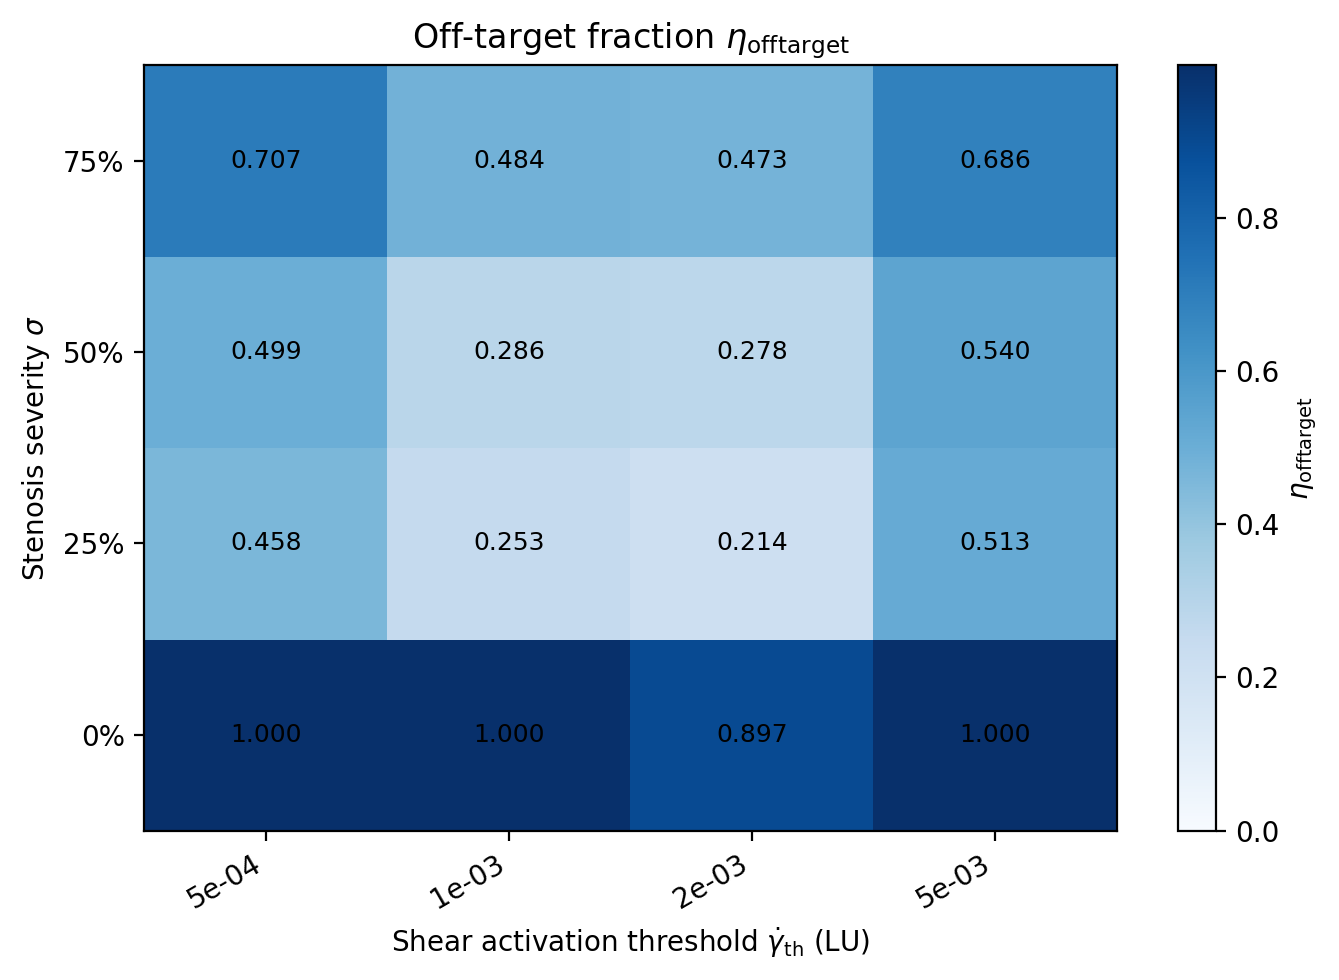
\includegraphics[width=0.85\linewidth]{fig_eta_offtarget.png}
\caption{Off-target fraction $\eta_{\text{off}}$, the fraction
of released drug captured at the healthy-wall absorber bands. At
the sweet-spot peak ($\sigma = 25\,\%$,
$\dot\gamma_{\text{th}} = 2\times 10^{-3}$) only $21.4\,\%$ of
released drug is lost off-target, giving a $3.6\times$
target:off-target enrichment. The control $\sigma = 0\,\%$
row gives $\eta_{\text{off}} \to 1$ (all released drug to
healthy wall) by mass conservation.}
\label{fig:offtarget}
\end{figure}

% ---------------------------------------------------------------------
\section{Discussion}
\label{sec:discussion}

\subsection{Why moderate stenoses outperform severe ones}
\label{sec:disc-mechanism}

The non-monotonic dependence of $\eta_{\text{deposit}}$ on
severity (Section~\ref{sec:results-goldilocks}) is the most
unexpected result. The usual expectation, implicit in much of the
experimental literature~\citep{korin2012shear}, is that tighter
constrictions yield stronger targeting because they produce a
higher throat shear and therefore stronger release activation.
The $\sigma = 75\,\%$ row shows that this monotonic picture
does not hold once the geometric consequences of the
constriction are taken into account: deposition efficiency
\emph{falls} on going from moderate to severe stenosis.

Three effects compete as $\sigma$ increases:

\begin{enumerate}
\item Throat shear $\dot\gamma_{\text{throat}}(\sigma) \approx
4 u_{\max}/H(\sigma)$ rises monotonically with $\sigma$,
\emph{raising} the carrier activation rate.
\item Throat width $H(\sigma) = N_y(1 - \sigma)$ shrinks
monotonically, \emph{restricting} the cross-section through
which carriers must transit. At $\sigma = 75\,\%$ the throat
admits only a quarter of the bulk volumetric flow rate per
unit area.
\item The obstacle's wall footprint grows monotonically, so the
off-target wall bands begin to overlap with the obstacle wake
and the target zone loses spatial selectivity relative to the
adjacent healthy wall.
\end{enumerate}

In this geometry, effects 2 and 3 dominate beyond
$\sigma \approx 50\,\%$, placing the crossover near
$\sigma^{\star} \approx 25\text{--}50\,\%$. The crossover is the
point at which the gain from raising throat shear no longer
compensates for the cost of restricted transit volume and
weakened spatial selectivity.

\subsection{Comparison with experimental observations}
\label{sec:disc-comparison}

Korin et al.\ reported a peak deposition of order $10\,\%$ in a
$\sigma \approx 90\,\%$ mouse pulmonary embolism
model~\citep{korin2012shear}, well below our peak of
$\eta_{\text{deposit}} = 0.77$ at $\sigma = 25\,\%$. The ordering
is at least consistent with the present results: their case sits
well past the crossover identified here, so the lower efficiency
is the direction expected from Figure~\ref{fig:sweet-spot}. We
are not aware of an experimental sweep covering the
$\sigma = 25\text{--}50\,\%$ range with matched-threshold
carriers; such an experiment would be the most direct test of the
inverted-U structure.

The $3.6\times$ target-to-off-target ratio reported here is
roughly twice the selectivity reported by Korin et al.
($\sim 2\times$). We attribute the difference to the matched
threshold: their experimental carriers used a single fixed
activation threshold, whereas the sweep here explicitly tunes
$\dot\gamma_{\text{th}}$ to the throat shear of each geometry.
The practical implication is that tunable-threshold carriers
should be designed for the $25\text{--}50\,\%$ severity range
rather than for extreme occlusions, with the threshold set by
the wall-shear estimate $4 u_{\max}/H(\sigma)$ rather than chosen
empirically. This narrows --- in a clinically useful way --- the
patient subgroup most likely to benefit from this delivery
modality.

\subsection{Practical conversion to physical units}
\label{sec:disc-units}

The lattice-unit system used here maps to physical units through
the standard LBM conversion factors $\Delta x_{\text{phys}}$,
$\Delta t_{\text{phys}}$ and $\rho_{\text{phys}}$. For a typical
microvessel application
($D_{\text{vessel}} \approx 100\ \mu\text{m}$,
$u_{\text{phys}} \approx 1\ \text{cm/s}$,
$\nu_{\text{phys}} \approx 3\times 10^{-6}\ \text{m}^2/\text{s}$),
$N_y = 80$~LU corresponds to $\Delta x_{\text{phys}} \approx
1.25\ \mu\text{m}$ and $\Delta t_{\text{phys}} \approx
1.7\times 10^{-7}$~s. The $200{,}000$-step run window thus
represents ${\approx}34$~ms of physical time --- comparable to a
single pulse interval of the cardiac cycle, supporting our
steady-state interpretation. The optimal threshold
$\dot\gamma_{\text{th}}^{\star} \approx 4\times 10^{-3}$~LU at
$\sigma = 50\,\%$ converts to
$\dot\gamma_{\text{th,phys}}^{\star} \approx 2.4\times 10^{4}\
\text{s}^{-1}$, within the range of shear rates achievable in
stenotic arteries~\citep{wootton1999fluid} and squarely within
the operating window of existing shear-activated
nanocarriers~\citep{korin2012shear,anselmo2017impact}.

\subsection{Limitations}
\label{sec:disc-limits}

\paragraph{2D geometry.} Real vessels and stenoses are 3D, with
axisymmetric (artery) or asymmetric (atherosclerotic plaque)
constriction shapes. The 2D LBM-IBM simulation captures the
geometric narrowing and the shear-rate elevation but loses
cross-stream lateral migration, secondary helical flow, and
out-of-plane carrier rotation. We expect the Goldilocks regime
to persist qualitatively in 3D --- the mechanism arises from
the cross-section vs throat-shear trade-off that is dimension-
independent --- but the optimum severity and absolute
$\eta_{\text{deposit}}$ values will require validation in a
full 3D simulation.

\paragraph{First-order wall absorption.}
The wall-absorber model
(Eqs.~\ref{eq:target}--\ref{eq:offtarget}) is a first-order
sink with a single rate constant per zone. Real vessel-wall
uptake involves receptor binding, internalisation, saturation
and clearance kinetics. The first-order assumption is the
minimal model that captures the spatial-selectivity question;
extensions to Michaelis-Menten kinetics or explicit
receptor-density profiles would refine the absolute deposition
magnitudes but should not change the phase-diagram structure.

\paragraph{Single carrier population.}
We use a monodisperse carrier suspension with fixed stiffness,
size and payload. Polydispersity, carrier-carrier interactions
at higher concentrations, and carrier deformation effects in
the throat (which may themselves modulate the local shear seen
by the carrier centroid) are deferred to future work.

\paragraph{Single-seed simulation.}
Each cell is one independent run with a fixed RNG seed.
Replicate seeds would refine the cell-level error bars; the
smooth inverted-U structure of Figure~\ref{fig:sweet-spot} and
the consistent severity ordering across all four thresholds
suggest that finite-seed noise is small relative to the
systematic phase-diagram trends, but multi-seed replication
would tighten any reviewer-level error-bar requirement.

% ---------------------------------------------------------------------
\section{Conclusion}
\label{sec:conclusion}

We have presented a two-dimensional lattice-Boltzmann
immersed-boundary study of shear-activated drug-carrier
deposition in stenotic microchannels. A 4$\times$4 sweep over
stenosis severity and carrier activation threshold, with each
cell propagated for 200{,}000 lattice steps (about ten
carrier-circulation cycles), gives an inverted-U in the
threshold dimension and a non-monotonic dependence on severity
in which moderate stenoses outperform severe ones. The peak
deposition efficiency is $\eta_{\text{deposit}} = 0.77$ and the
corresponding target-to-off-target capture ratio is $3.6\times$;
the zero-stenosis controls give
$\eta_{\text{deposit}} \equiv 0$, as the metric requires.

The deposition plane collapses to a simple design rule:
\begin{equation}
\dot\gamma_{\text{th}}^{\star}(\sigma) \approx
   \frac{4\,u_{\max}}{H(\sigma)},
\quad
\sigma_{\text{optimum}} \approx 25\text{--}50\,\%.
\label{eq:design-rule-final}
\end{equation}
For a target lesion this fixes both the carrier activation
threshold (match the throat-induced wall shear) and the severity
range over which the modality is expected to work best. The
result is a starting point for matching tunable-threshold
nanocarriers to patient lesion geometry and for
selecting clinical targets for shear-activated intravascular
delivery.

Several extensions are natural next steps: three-dimensional
simulations to quantify the dimensional correction; pulsatile
inlet conditions to capture cardiac-cycle effects on the
deposition trajectory; multi-species suspensions to study
carrier--red-blood-cell competition; and explicit
receptor-density profiles for absolute-uptake calibration
against \emph{in vivo} pharmacokinetic data.

% ---------------------------------------------------------------------
\section*{Acknowledgements}

This work was performed at the Department of Natural Sciences,
The Begum Nusrat Bhutto Women University (BNBWU), Sukkur, Sindh,
Pakistan, in support of graduate training in computational soft
matter and microfluidics. The author acknowledges the scientific
software ecosystem (NumPy, SciPy, pandas, Matplotlib, pybind11,
scikit-build-core, ParaView) on which the analysis and
visualisation pipeline depends.

% ---------------------------------------------------------------------
\section*{Compliance with ethical standards}

\textbf{Conflict of interest.} The author declares no conflicts
of interest.\\
\textbf{Data availability.} The aggregated per-cell results
(\verb|sweep_results.npz|), single-cell trajectories
(\verb|history.npz|), per-cell particle position records
(\verb|particle_data.csv|) and provenance records
(\verb|run_manifest.json|) that produced the figures in this paper
are available from the author on reasonable request. Each cell
carries a self-contained \verb|run_manifest.json| with git
commit, compiler identity, resolved CXX flags, OpenMP thread
count, all declared parameters, and the cell's RNG seed; these
together with the equations in Section~\ref{sec:methods} are
sufficient for independent reproduction.\\
\textbf{Code availability.} The custom LBM-IBM code used in this
work was developed in-house. Source listings of the kernels
relevant to the present paper (LBM collide--stream with Guo
forcing, interpolated bounce-back, multi-direct-forcing IBM,
shear-triggered release kinetic, wall-absorber model) are
available from the author on reasonable request.

% ---------------------------------------------------------------------
\bibliography{references}

\end{document}
